\chapter{Prototypische Implementierung}\label{section:prototypische-implementierung}

Für die Prototypische Implementierung der IDE wurde ein Fokus auf die Programmierung von AVR Microcontrollern \cite{noauthor_avr_nodate} gelegt. Hierbei wurde für Beispielzwecke der ATmega2560 \cite{noauthor_atmega2560_nodate} genutzt. Dadurch wird die Betrachtung aller in den Anforderungen beschriebenen Funktionen ermöglicht. In \autoref{section:prototypische-implementierung:code-editor} wird zunächst die Auswahl eines passenden Code Editors beschrieben. Danach wird in \autoref{section:prototypische-implementierung:experimentkonfiguration} eine Experimentkonfiguration beschrieben, die in den nachfolgenden Abschnitten um weitere Laborgeräte und CrossLab-Services erweitert wird. Daraufhin wird in \autoref{section:prototypische-implementierung:crosslab-kompatibilität} die Herstellung der CrossLab-Kompatibilität erläutert. Darauf aufbauend wird in \autoref{section:prototypische-implementierung:kollaboration} die Implementierung der Kollaborationsmechanismen dargelegt. In \autoref{section:prototypische-implementierung:dateisystem} wird die Implementierung des Dateisystems beschrieben. \autoref{section:prototypische-implementierung:kompilierung-und-programmierung} befasst sich mit der Einbindung eines Compilers für die AVR Microcontroller sowie deren Programmierung. Daraufhin wird in \autoref{section:prototypische-implementierung:debugging} die Einbindung eines entsprechenden Debuggers erläutert. Danach wird in \autoref{section:prototypische-implementierung:testen} die Implementierung der Erstellung und Ausführung von Testfällen beschrieben. Schließlich wird in \autoref{section:prototypische-implementierung:language-server} die Anbindung eines passenden Language Servers dargelegt. Der komplette Quellcode, der im Rahmen dieser Arbeit entstanden ist, kann in \cite{lassertos_lassertosmasterarbeit_2025} eingesehen werden.

\section{Code Editor}\label{section:prototypische-implementierung:code-editor}

% \begin{note}
%     \textbf{Notizen:}
%     \begin{itemize}
%         \item \autoref{requirement:Erweiterbarkeit}, \autoref{requirement:Kostenlos nutzbar}, \autoref{requirement:Komplett im Browser nutzbar} und \autoref{requirement:Nur CrossLab-Nutzerkonto nötig}
%         \item Betrachtung verschiedener Optionen: \\ Eigenimplementierung, Visual Studio Code, Eclipse Theia und OpenSumi
%         \item Begründung warum Implementierung über VSCode Extensions
%         \item Begründung warum VSCode als Code Editor
%         \item Ggf. nicht als eigenes Unterkapitel
%     \end{itemize}
% \end{note}

Es gibt viele verschiedene Code Editoren, die für die prototypsische Implementierung der IDE verwendet werden können. So kann ein bereits vorhandener Code Editor wie z.B. Ace oder der Monaco Editor genutzt werden um diese in ein eigenes Benutzerinterface einzubinden. Dies ermöglicht, mit Ausnahme einer Eigenimplementierung des Code Editors, die größtmögliche Kontrolle über die Implementierung der IDE. Allerdings wird dadurch auch der Implementierungsaufwand stark erhöht. Eine weitere Option ist die Nutzung von Code Editoren, die bereits etablierte Benutzerinterfaces und Erweiterungsmöglichkeiten besitzen. Beispiele hierfür sind \ac{VSCode} \cite{noauthor_vscode_nodate}, Eclipse Theia \cite{noauthor_theia_nodate} und OpenSumi \cite{noauthor_opensumi_nodate}. Hierbei bieten Theia und OpenSumi neben der Erweiterbarkeit durch die VSCode Extension API \cite{noauthor_vscode-extension-api_nodate} auch noch weitere Schnittstellen an, die zur Erweiterung und Anpassung von grundlegenden Funktionen genutzt werden können. Durch die Nutzung bereits vorhandener und etablierter Benutzerinterfaces und Erweiterungsmöglichkeiten kann die Entwicklung der IDE stark vereinfacht werden. Dabei ist zu beachten, dass ggf. nicht alle erwünschten Änderungen über die angebotenen Schnittstellen umgesetzt werden können. Zudem entsteht durch die Nutzung von tiefgreifenden Schnittstellen von Theia und OpenSumi eine Bindung an das jeweilige Framework, wodurch ein späterer Wechsel auf eine andere Plattform erschwert wird. Aus diesen Gründen wird eine Implementierung über die VSCode Extension API angestrebt. Diese wird von allen drei genannten Möglichkeiten unterstützt, wodurch die entwickelte Lösung auf alle anwendbar sein sollte. Während der prototypischen Implementierung wurde \ac{VSCode} als Code Editor für die IDE verwendet.
\section{Experimentkonfiguration}\label{section:prototypische-implementierung:experimentkonfiguration}

\begin{note}
    \textbf{Notizen:}
    \begin{itemize}
        \item Beschreibung der Experimentkonfiguration
        \item Beschreibung des virtuellen Modells
        \item Beschreibung der Microcontroller Simulation
    \end{itemize}
\end{note}
\input{content/06_implementierung/063_crosslab_kompatibilität.tex}
\section{Kollaboration}\label{section:prototypische-implementierung:kollaboration}

% \begin{note}
%     \textbf{Notizen:}
%     \begin{itemize}
%         \item Kurze Begründung warum Yjs für die Implementierung ausgewählt wurde
%         \item Beschreibung der Implementierung mit Yjs
%               \begin{itemize}
%                   \item CollaborationProvider
%                   \item CollaborationTypes
%               \end{itemize}
%     \end{itemize}
% \end{note}

Um das in \autoref{section:konzeption:kollaboration} beschriebene Konzept zur Bereitstellung von Echtzeit-Kollaboration innerhalb von Experimenten umzusetzen, wurden der Collaboration Service und eine Erweiterung für die IDE implementiert. Diese Erweiterung wird im Folgenden als \textit{Collaboration Erweiterung} bezeichnet.

Die Implementierung des Collaboration Service ist nach dem in \autoref{section:konzeption:kollaboration} vorgestellten Konzept erfolgt. Als Synchronisationsmethode wurde die Bibliothek Yjs \cite{noauthor_yjs_nodate} verwendet, welche auf dem Konzept von \acp{CRDT} basiert\todo{Erklärungssatz}. Alle Teilnehmer einer Kollaborationssitzung sind in Yjs gleichberechtig. Das bedeutet, dass alle Nutzer sowohl als Producer als auch als Consumer auftreten. Dementsprechend wurde zunächst nur ein Collaboration Service Prosumer implementiert, der beide Rollen abdeckt. Für die Implementierung der verschiedenen kollaborativen Datentypen wurden die von Yjs angebotenen Datentypen \texttt{Map}, \texttt{Array} und \texttt{Text} verwendet. Dabei können diese direkt auf Objekte, Arrays und Strings abgebildet werden. Für die Implementierung der restlichen kollaborativen Datentypen wurde \texttt{Text} verwendet, wobei der entsprechende Datentyp über ein zusätzliches Attribut festgelegt wird, um die Zuordnung zu ermöglichen. Die Möglichkeit Attribute an den Datentyp \texttt{Text} anzufügen, welche entsprechend synchronisiert werden, wird bereits von Yjs unterstützt.

Die Collaboration Erweiterung bietet einen Collaboration Service Prosumer an. Dieser kann von anderen Erweiterungen verwendet werden, um entsprechende Räumen beizutreten. Dadurch kann die Implementierung von spezifischen kollaborativen Funktionen durch die entsprechenden Erweiterungen vorgenommen werden. Aktuell wird nur Yjs als Synchronisationsmethode unterstützt.

In der betrachteten Experimentkonfiguration wird zur Veranschaulichung der Kollaboration eine weitere IDE hinzugefügt. Beide IDEs erhalten einen Collaboration Service Prosumer. Es wird eine Verbindung zwischen den beiden IDEs über den Collaboration Service hinzugefügt.
\section{Dateisystem}\label{section:prototypische-implementierung:dateisystem}

\begin{figure}[tbp]
    \centering
    \begin{tikzpicture}
        \begin{class}[text width=6cm]{FilesystemServiceProducer}{0,0}
            \operation{+ onCreateDirectory()}
            \operation{+ onDelete()}
            \operation{+ onMove()}
            \operation{+ onCopy()}
            \operation{+ onExists()}
            \operation{+ onStat()}
            \operation{+ onReadDirectory()}
            \operation{+ onReadFile()}
            \operation{+ onWriteFile()}
            \operation{+ onRegisterWatcher()}
            \operation{+ onUnregisterWatcher()}
        \end{class}
        \begin{class}[text width=6cm]{FilesystemServiceConsumer}{7,0}
            \operation{+ createDirectory()}
            \operation{+ delete()}
            \operation{+ move()}
            \operation{+ copy()}
            \operation{+ exists()}
            \operation{+ stat()}
            \operation{+ readDirectory()}
            \operation{+ readFile()}
            \operation{+ writeFile()}
            \operation{+ registerWatcher()}
            \operation{+ unregisterWatcher()}
            \operation{+ onWatcherEvent()}
        \end{class}
    \end{tikzpicture}
    \caption{Klassendiagramm Filesystem Service}
    \label{figure:klassendiagramm-dateisystem-service}
\end{figure}

\begin{figure}[tbp]
    \centering
    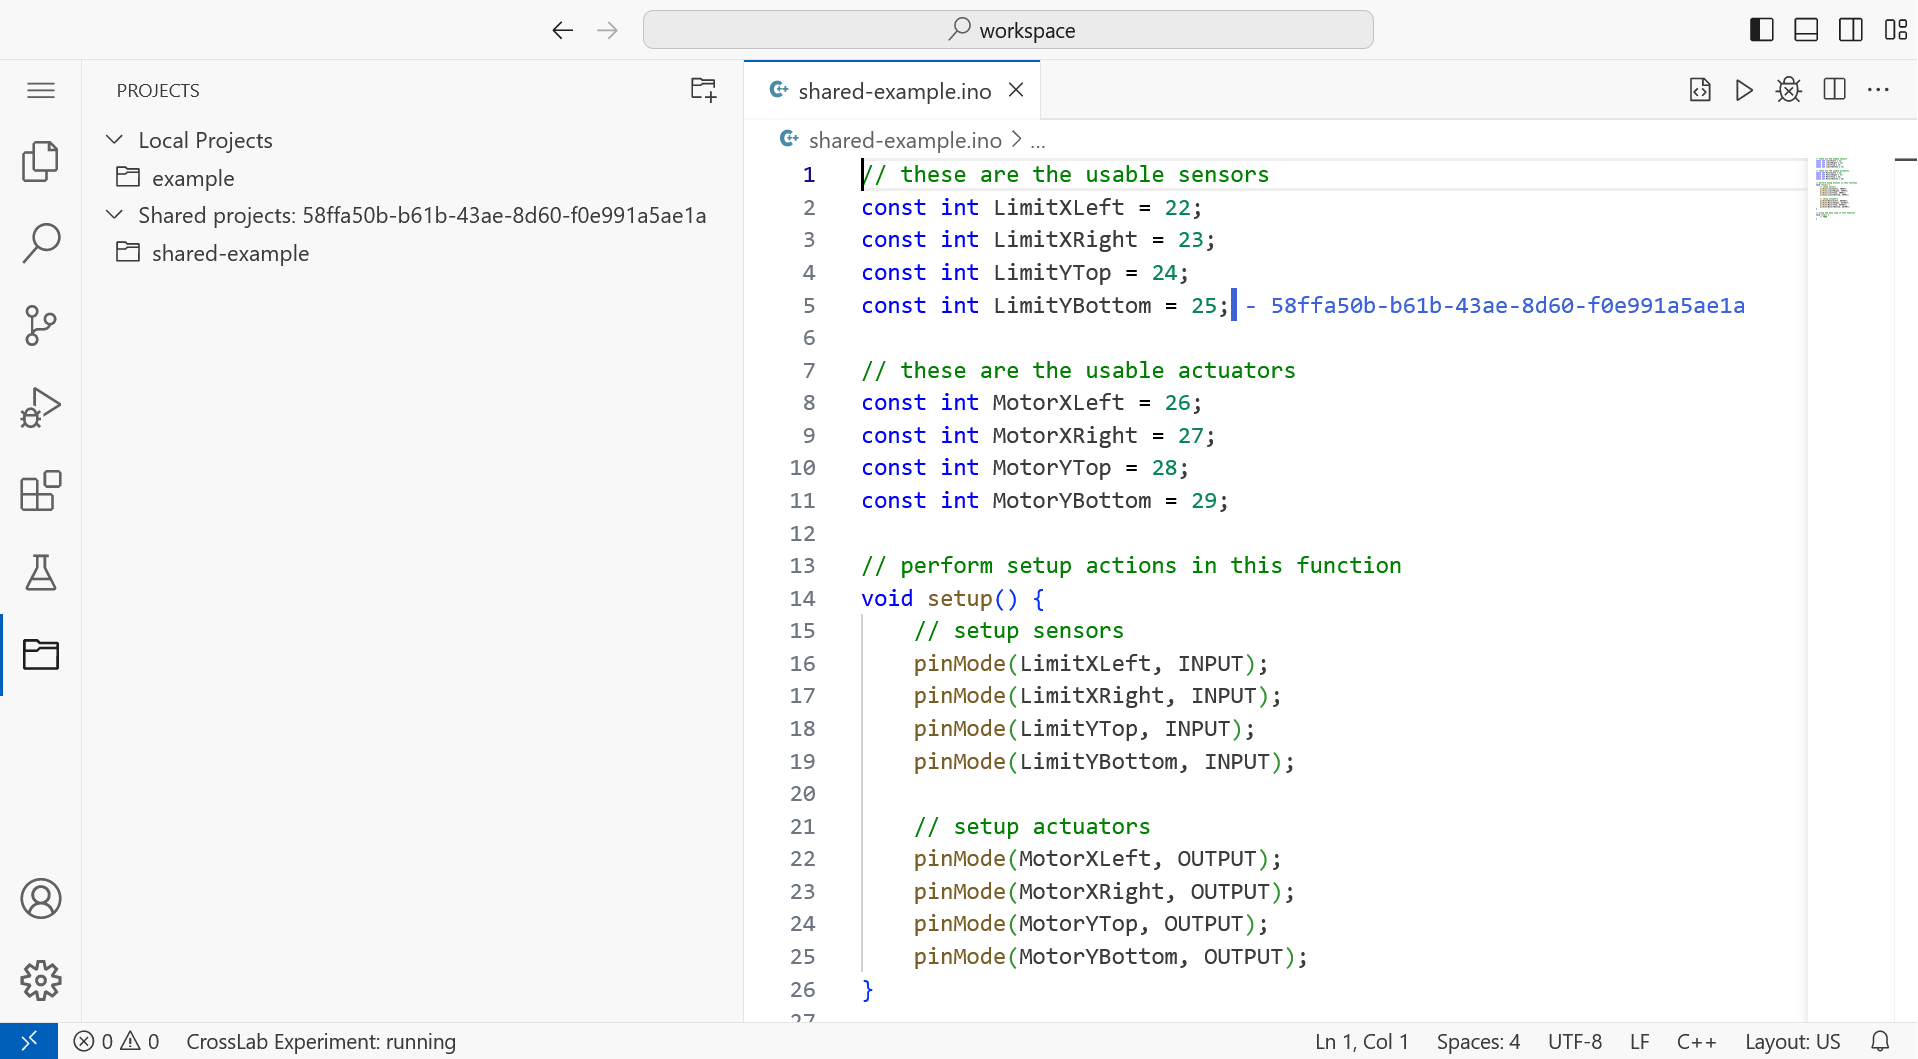
\includegraphics[trim={0 3px 0 0},clip,width=\textwidth]{images/projects-shared.png}
    \caption{Benutzerinterface der Projektverwaltung}
    \label{figure:benutzerinterface:dateisystem}
\end{figure}

Um die in \autoref{section:konzeption:dateisystem} beschriebenen Konzepte für die Bereitstellung und Nutzung von Dateisystemen umzusetzen, wurden der Filesystem Service sowie eine entsprechende Erweiterung für die IDE entwickelt. Diese Erweiterung wird im Folgenden als \textit{Filesystem Erweiterung} bezeichnet.

In \autoref{figure:klassendiagramm-dateisystem-service} ist ein Klassendiagramm für den Filesystem Service dargestellt. Der Filesystem Service Consumer besitzt die in \autoref{section:konzeption:dateisystem} genannten Funktionen zur Interaktion mit dem vom Filesystem Service Producer angebotenen Dateisystem. Der Filesystem Service Producer ermöglicht die Registrierung von Event-Handlern um auf die verschiedenen Anfragen reagieren zu können. Dadurch kann die Implementierung an das angebotene Dateisystem angepasst werden.

Die Filesystem Erweiterung ist für die Bereitstellung des integrierten Dateisystems und die Ermöglichung des kollaborativen Arbeitens an Programmen verwantwortlich. Für das integrierte Dateisystem wurde ein projektbasierter Ansatz gewählt. Dabei besitzen Nutzer mehrere verschiedene \textit{Projektordner}, deren direkte Unterordner als \textit{Projekte} bezeichnet werden. In der aktuellen Implementierung gibt es standardmäßig den Projektordner \texttt{/projects}. Die Projektordner sowie die enthaltenen Projekte werden dem Nutzer über ein entsprechendes Benutzerinterface angezeigt. Über dieses kann der Nutzer Projekte erstellen, öffnen, umbenennen und löschen. Für die Einbindung des Dateisystems wurde das Interface \texttt{FileSystemProvider} der VSCode Extension API implementiert. Für die Bereitstellung der Dateisystem-Funktionen können unterschiedliche \textit{Subprovider} verwendet werden. In der aktuellen Implementierung stehen dabei Subprovider für In-Memory, die Indexed Database API sowie den Filesystem Service zur Verfügung. Dabei werden standardmäßig der In-Memory Subprovider sowie der Indexed Database Subprovider für die persistente Speicherung der Projekte im Pfad \texttt{/projects} verwendet. Allerdings können der standardmäßig benutzte Subprovider sowie die Subprovider für bestimmte Pfade angepasst und neue Subprovider hinzugefügt werden. Weiterhin wurden auch die Schnittstellen \texttt{FileSearchProvider} und \texttt{TextSeachProvider} der VSCode Extension API implementiert, um es Nutzern zu ermöglichen, nach Dateien und Texten innerhalb des aktuellen Projekts zu suchen. Für das Benutzerinterface wurde eine \texttt{TreeView} verwendet, deren Daten über einen entsprechenden \texttt{TreeDataProvider} bereitgestellt werden. Das von der Filesystem Erweiterung bereitgestellte Benutzerinterface zur Verwaltung der Projekte ist in \autoref{figure:benutzerinterface:dateisystem} dargestellt. Dieses enthält auch bereits ein geteiltes Projekt, um die Darstellung unterschiedlicher Projektordner hervorzuheben.

Beim Öffnen eines neuen Ordners wird VSCode standardmäßig neugeladen. Dadurch werden auch alle Erweiterungen beendet und neugestartet, was dazu führt, dass das laufende Experiment beendet wird. Um dies zu vermeiden, muss der Wechsel von Projekten über einen anderen Mechanismus geschehen. Dazu wurde zunächst ein Pfad festgelegt, welcher standardmäßig von der IDE geöffnet wird. Im Falle der prototypischen Implementierung wurde der Pfad \texttt{/workspace} ausgewählt. Dieser Pfad nutzt standardmäßig einen In-Memory Subprovider. Sollte der Nutzer nun ein Projekt öffnen, wird von diesem Moment an der Pfad \texttt{/workspace} in allen URLs durch den Pfad des geöffneten Projektes ersetzt. Dadurch wird kein Neuladen der IDE ausgelöst und Nutzer können zwischen ihren Projekten wechseln. Das Umschreiben der Pfade führt allerdings zu Problemen beim Kopieren, Ausschneiden und Einfügen von Ordnern und Dateien. Daher müssen die entsprechenden Kommandos überschrieben werden, um die erwartete Funktionalität zu gewährleisten.

Um das Teilen von Projekten sowie das gleichzeitige Bearbeiten dieser zwischen Nutzern innerhalb eines Experiments zu ermöglichen, wurde eine entsprechende Komponente implementiert. Diese nutzt den \texttt{FileSystemProvider} sowie den von der Collaboration Erweiterung bereitgestellten Collaboration Service Prosumer. Über diesen wird ein enstsprechender Raum erstellt. Zu Beginn wird kein Projekt geteilt. Sobald ein Nutzer ein Projekt teilt, wird es zu dem geteilten Objekt des Raums hinzugefügt. Weiterhin werden auch Funktionen registriert, die auf Änderungen innerhalb des Projekts reagieren. Andere Nutzer die an der Kollaboration teilnehmen, können dann das geteilte Projekt über das bereitgestellte Benutzerinterface aufrufen. Alle Änderungen an Dateien und Ordnern werden zwischen den Nutzern synchronisiert. Weiterhin wird die aktuelle Position eines Nutzers innerhalb einer Datei über dessen Zustandsinformationen geteilt. Diese Position wird dann bei anderen Nutzern innerhalb derselben Datei markiert (siehe \autoref{figure:benutzerinterface:dateisystem}). Wenn der Besitzer des Projekts das Teilen beendet, wird das Projekt für alle anderen Nutzer geschlossen. Geteilte Projekte besitzen Pfade der Form \texttt{/shared/\{\{user\_id\}\}/\{\{project\_name\}\}}, wobei der Pfad \texttt{/shared} ein In-Memory Dateisystem verwendet. Die Projektordner \texttt{/shared/\{\{user\_id\}\}} werden automatisch erstellt, wenn ein Nutzer dem entsprechenden Raum beitritt.

Der betrachteten Experimentkonfiguration werden keine neuen Laborgeräte hinzugefügt. Die IDEs werden um einen Filesystem Service Consumer erweitert, der die Anbindung von weiteren Dateisystemen ermöglicht. Außerdem bieten die IDEs auch einen Filesystem Service Producer an, um die Nutzung des integrierten Dateisystems durch andere Laborgeräte zu ermöglichen (siehe \autoref{figure:experimentkonfiguration:dateisystem}). Zudem wird ein neuer Raum für die Verbindungen der Collaboration Service Prosumer hinzugefügt, um das Teilen von Projekten zu ermöglichen.
\section{Kompilierung}\label{section:prototypische-implementierung:kompilierung}

\begin{note}
    \textbf{Notizen:}
    \begin{itemize}
        \item Begründung warum Arduino CLI für die Implementierung genutzt wurde
        \item Beschreibung der Anbindung der Arduino CLI als Laborgerät
        \item (Angabe der Rückgabeformate?)
        \item Ggf. Beschreibung der Benutzerinterfaces + Screenshots
    \end{itemize}
\end{note}

Für die Kompilierung wurde in der prototypischen Implementierung das Arduino Command Line Interface \cite{noauthor_arduino-cli_nodate} verwendet. Dieses nutzt intern den Compiler \ac{GCC} \cite{noauthor_gcc_nodate}. Neben der Kompilierung des Quellcodes werden auch Arduino spezifische Vorverarbeitungsschritte durchgeführt. Dadurch können Nutzer auch ggf. ihnen bereits bekannte Arduino Funktionen wie z.B. \texttt{digitalWrite} und \texttt{digitalRead} nutzen. Im Allgemeinen sollte dadurch die Programmierung der Microcontroller für die Nutzer vereinfacht werden. Um die Arduino-cli zur Kompilierung innerhalb eines Experiments nutzen zu können muss diese als ein entsprechendes Laborgerät bereitgestellt werden. Dafür wurde ein cloud-instanziierbares Laborgerät entwickelt. Dieses bietet einen entsprechenden Kompilierungs Service Producer an, welcher während einem Experiment mit der IDE verbunden werden kann. Das instanziierte Laborgerät nimmt die entsprechenden Kompilieranfragen entgegen und bearbeitet diese. Sollte die Kompilierung erfolgreich sein wird eine entsprechende Antwort mit dem Ergebnis der Kompilierung an die IDE gesendet. Im Fehlerfall wird die Fehlermeldung in der Antwort mitgesendet.

Um die Kompilierung aus der IDE starten zu können wurde eine entsprechende Erweiterung entwickelt. Diese fügt zwei Bedienelemente hinzu. Eine Schaltfläche zur Kompilierung des aktuellen Projekts sowie eine Taste zum Kompilieren und Hochladen des aktuellen Projekts. Die erste Schaltfläche kann dazu genutzt werden um zu überprüfen ob das aktuelle Projekt kompiliert werden kann und um die entsprechenden Mitteilungen vom Compiler zu erhalten. Die zweite Schaltfläche führt auch eine Kompilierung des aktuellen Projekts durch und zeigt entsprechende Rückmeldungen an. Sollte die Kompilierung erfolgreich sein wird anschließend das Ergebnis dieser an die zu programmierende Steuereinheit gesendet. In einer kollaborativen Sitzung ist das Kompilieren von Projekten stets erlaubt. Allerdings wird das Hochladen von Projekten deaktiviert falls ein anderer Nutzer aktuell ein Projekt auf die Steuereinheit hochlädt oder falls die Steuereinheit in einer Debug-Sitzung verwendet wird.
\section{Debugging}\label{section:prototypische-implementierung:debugging}

\begin{figure}[tbp]
    \centering
    \resizebox{\textwidth}{!}{
        \begin{tikzpicture}
            \begin{class}[text width=7.5cm]{DebuggingAdapterServiceProducer}{0,0}
                \operation{+ sendMessageDAP()}
                \operation{+ onStartSession()}
                \operation{+ onJoinSession()}
                \operation{+ onMessageDAP()}
            \end{class}
            \begin{class}[text width=7.5cm]{DebuggingAdapterServiceConsumer}{8,0}
                \operation{+ sendMessageDAP()}
                \operation{+ startSession()}
                \operation{+ joinSession()}
                \operation{+ onMessageDAP()}
            \end{class}
            \begin{class}[text width=7.5cm]{DebuggingTargetServiceProducer}{0,-3.5}
                \operation{+ sendDebuggingMessage()}
                \operation{+ onStartDebugging()}
                \operation{+ onEndDebugging()}
                \operation{+ onDebuggingMessage()}
            \end{class}
            \begin{class}[text width=7.5cm]{DebuggingTargetServiceConsumer}{8,-3.5}
                \operation{+ sendDebuggingMessage()}
                \operation{+ startDebugging()}
                \operation{+ endDebugging()}
                \operation{+ onDebuggingMessage()}
            \end{class}
        \end{tikzpicture}
    }
    \caption{Klassendiagramm Debugging Services}
    \label{figure:klassendiagramm-debugging-services}
\end{figure}

Für die Bereitstellung der Debug-Funktionen wurde in der prototypischen Implementierung der \textit{\ac{GDB}} \cite{noauthor_gdb_nodate} verwendet. Dieser erlaubt das Debuggen von Microcontrollern und besitzt zudem einen integrierten Debug Adapter. Um \ac{GDB} in Experimenten nutzen zu können, wurde ein cloud-instanziierbares Laborgerät entwickelt. Dieses stellt einen Debugging Adapter Service Producer und einen Debugging Target Service Consumer für die Kommunikation mit der IDE sowie der zu debuggenden Steuereinheit bereit.

In \autoref{figure:klassendiagramm-debugging-services} ist ein Klassendiagramm für den Debugging Adapter Service und den Debugging Target Service dargestellt. Hierbei besitzt der Debugging Adapter Service Consumer die Funktionen \texttt{startSession()} und \texttt{joinSession()}, um eine neue Debug-Sitzung zu starten oder einer laufenden beizutreten. Der Debugging Adapter Service Producer löst entsprechende Events aus, die über Event-Handler behandelt werden können. Sowohl der Debugging Adapter Service Consumer als auch der Debugging Adapter Service Producer besitzen Funktionen, um DAP-Nachrichten zu versenden und auf diese zu reagieren. Der Debugging Target Service Consumer besitzt die Funktionen \texttt{startDebugging()} und \texttt{endDebugging()}, um den Beginn bzw. das Ende einer Debug-Sitzung zu signalisieren. Auch hier löst der Debugging Target Service Producer entsprechende Events aus, die über Event-Handler behandelt werden können. Sowohl der Debugging Target Service Consumer als auch der Debugging Target Service Producer besitzen Funktionen, um Debug-Nachrichten zu versenden und auf diese zu reagieren.

Wenn ein Nutzer eine Debug-Sitzung startet, wird über den Debugging Adapter Service eine entsprechende Nachricht an das Laborgerät des Debuggers gesendet. Diese Nachricht beinhaltet das aktuelle Projekt des Nutzers. Dieses benötigt der Debugger während der Debug-Sitzung, weshalb es für die Dauer der Debug-Sitzung in einem entsprechenden Ordner auf dem Dateisystem hinterlegt wird. Weiterhin wird das Projekt an den Compiler gesendet, wobei für die Ermöglichung des Debuggens spezielle Einstellungen vorgenommen werden müssen. Das Ergebnis der Kompilierung wird dann über den Debugging Target Service an die Steuereinheit gesendet, wodurch der Steuereinheit gleichzeitig der Beginn einer Debug-Sitzung mitgeteilt wird. Weiterhin wird der Debugger selbst gestartet, wobei der tatsächliche Start der Debug-Sitzung erst durch die Nachrichten des \ac{DAP} geschieht. Nachdem alle Vorbereitungen getroffen wurden und eine Antwort von der Steuereinheit empfangen wurde, wird eine Antwort an die IDE gesendet. Die Antwort enthält den Kennzeichner der Debug-Sitzung sowie Einstellungen für diese. Im Falle der prototypischen Implementierung werden hierbei der Kennzeichner der Debug-Sitzung, das Debug-Ziel sowie der Pfad des kompilierten Programms als Einstellungen übergeben. Diese werden dann von der IDE beim Start des \ac{DAP} verwendet.

Damit das \ac{DAP} korrekt ausgeführt werden kann, muss eine Umschreibung der URIs vorgenommen werden, da die Dateien des Nutzers und des Debuggers unterschiedliche URIs besitzen. Außerdem gibt es Dateien, die nur auf dem Dateisystem des Debuggers vorhanden sind, wie z.B. Bibliotheken. Alle URIs, die von der IDE gesendet werden, beginnen entweder mit \texttt{crosslabfs:/workspace} für Dateien innerhalb eines Projekts oder mit \texttt{crosslab-remote:} für Dateien innerhalb des Dateisystems des Debuggers. Bei Ersteren wird das genannte Präfix durch den lokalen Pfad des Projektes auf dem Dateisystem des Debuggers ersetzt, während bei Zweiteren das Präfix gelöscht wird. Bei Nachrichten vom Debugger an die IDE werden Dateien innerhalb des Projekts wieder auf URIs beginnend mit \texttt{crosslabfs:/workspace} abgebildet, während alle anderen Dateien das Präfix \texttt{crosslab-remote:} erhalten.

Um das kollaborative Debuggen innerhalb eines Experiments zu unterstützen, müssen einige Nachrichten des \ac{DAP} speziell behandelt werden. Dazu gehören die Nachrichten für Breakpoints, Stacktraces, das Starten und Stoppen des Programms sowie das Beenden der Debug-Sitzung. Wenn Nutzer einer Debug-Sitzung beitreten, schicken sie zunächst nur ihre lokalen Breakpoints über eine \texttt{SetBreakpoints}-Anfrage. Damit nicht die Breakpoints der anderen Nutzer gelöscht werden, müssen diese entsprechend zu dieser Nachricht hinzugefügt werden. Dafür werden die Breakpoints aller Nutzer separat verwaltet. Außerdem müssen alle Events gespeichert werden, um diese beitretenden Nutzern schicken und den aktuellen Zustand der Debug-Sitzung herstellen zu können. Allgemein werden Events, die vom Debug Adapter ausgegeben werden, an alle Nutzer einer Debug-Sitzung gesendet. Wenn ein Nutzer das Programm startet oder fortsetzt, muss ein \texttt{Continued}-Event an die anderen Nutzer gesendet werden. Bei Breakpoints und Stacktraces muss darauf geachtet werden, dass die URIs für Dateien des Debuggers entsprechend angepasst werden, damit die IDE diese öffnen kann. Wenn der Ersteller der Debug-Sitzung diese beendet, so wird sie für alle Nutzer beendet. Sollte ein anderer Nutzer die Debug-Sitzung beenden, so wird sie nur für diesen Nutzer selbst beendet.

\begin{figure}[tbp]
    \centering
    \begin{tikzpicture}
        \node[anchor=south west,inner sep=0] at (0,0) {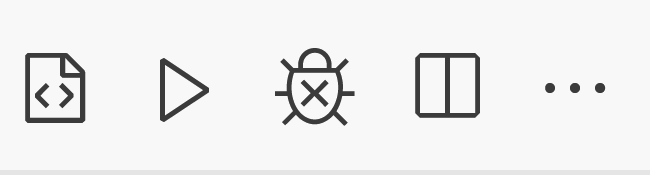
\includegraphics[trim={8.5cm 0 9.1cm 0},clip,width=0.1\textwidth]{images/symbols.png}};
        \node[anchor=south west,inner sep=0] at (2,0) {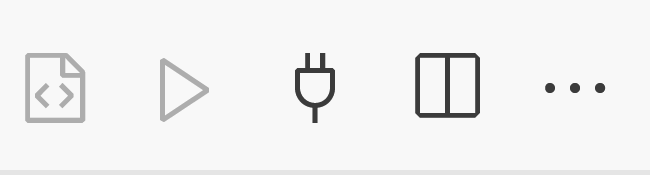
\includegraphics[trim={8.5cm 0 9.1cm 0},clip,width=0.1\textwidth]{images/symbols-join.png}};
        \draw[orange,ultra thick,rounded corners] (0.2,0.2) rectangle (1.35,1.55);
        \draw[blue!60,ultra thick,rounded corners] (2.2,0.2) rectangle (3.35,1.55);
        \node[orange] at (-2.8,0.75) {Starten einer Debug-Sitzung};
        \node[blue!60] at (6.5,0.75) {Beitreten einer Debug-Sitzung};
    \end{tikzpicture}
    \caption{Schaltflächen für das Starten und Beitreten einer Debug-Sitzung}
    \label{figure:benutzerinterface:symbole-debugging}
\end{figure}

\begin{figure}[tbp]
    \centering
    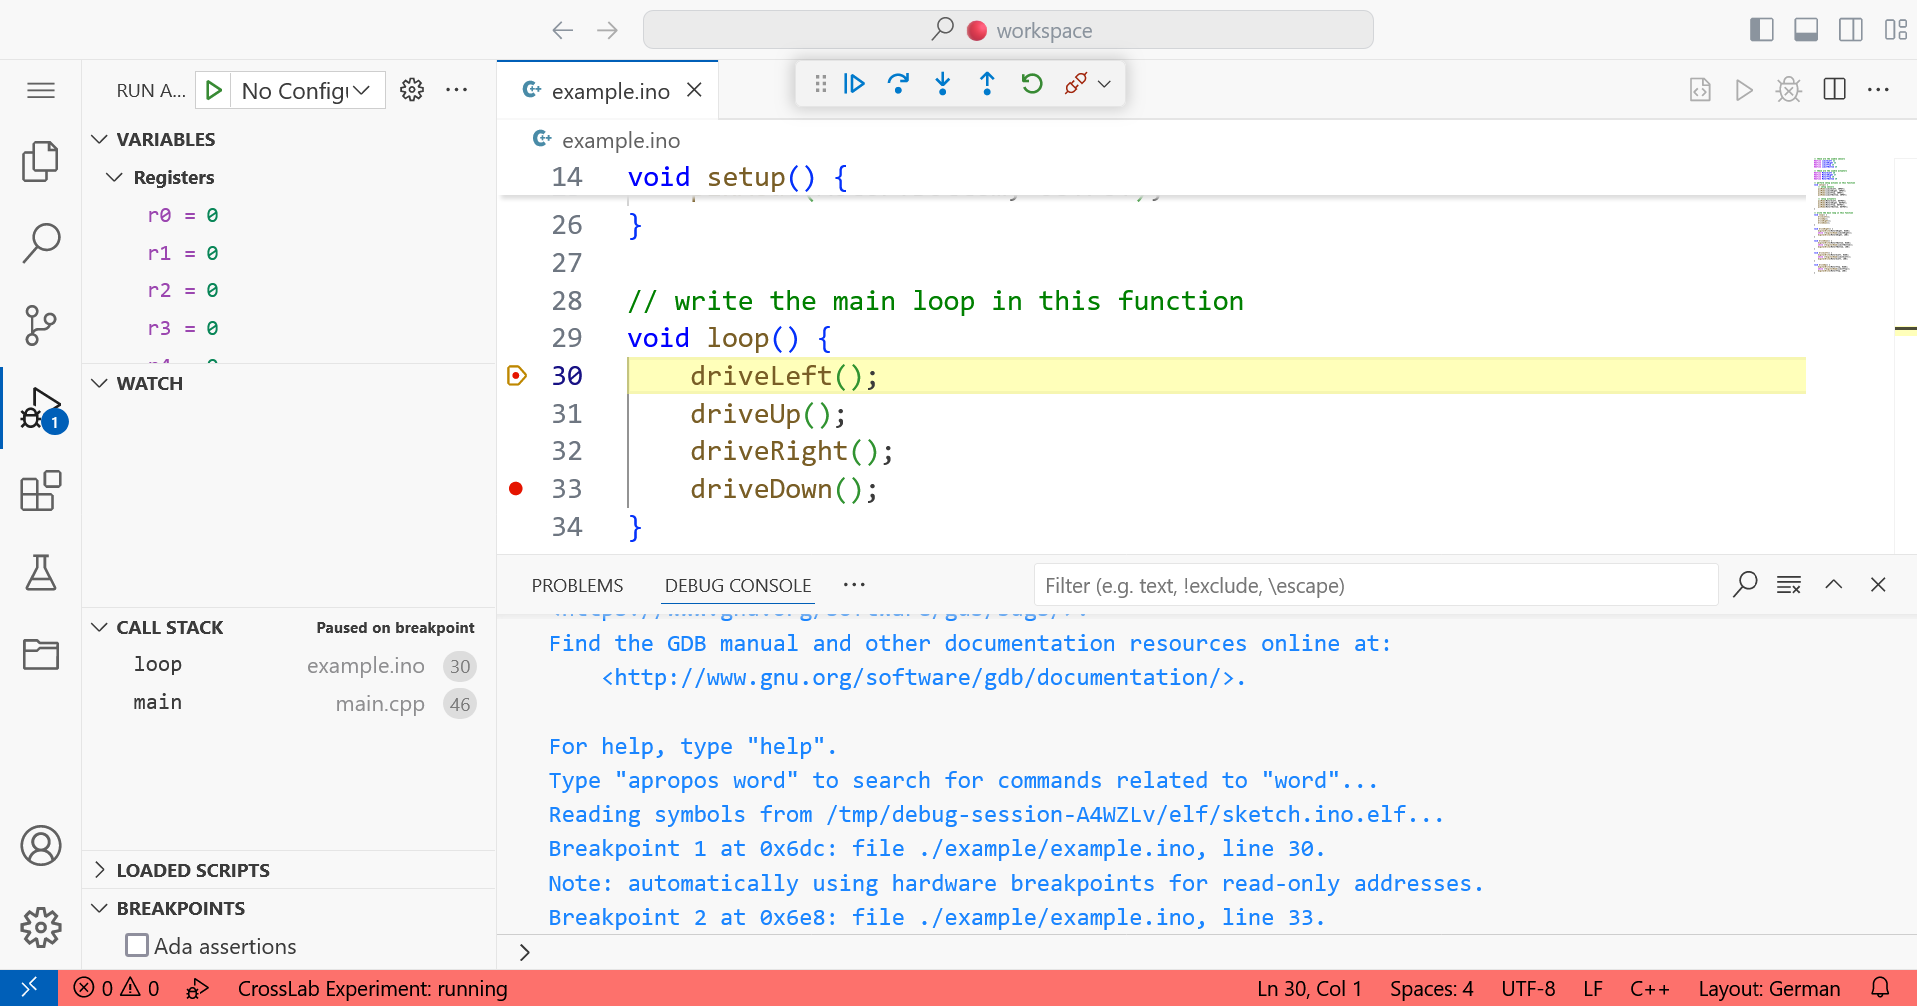
\includegraphics[trim={0 3px 0 0},clip,width=\textwidth]{images/debugging.png}
    \caption{Benutzerinterface der IDE während einer aktiven Debug-Sitzung}
    \label{figure:benutzerinterface:debugging}
\end{figure}

Für die Einbindung in die IDE wurde eine entsprechende Erweiterung entwickelt. Diese wird im Folgenden als \textit{Debugging Erweiterung} bezeichnet und fügt einen Debugging Adapter Service Consumer hinzu. Die Debugging Erweiterung beinhaltet zudem Implementierungen der Schnittstellen \texttt{DebugAdapter}, \texttt{DebugAdapterDescriptorFactory} und \texttt{DebugConfigurationProvider}. Mithilfe dieser Schnittstellen kann bereits ein Großteil der Funktionalität implementiert werden. Weiterhin werden auch Bedienelemente zum Starten bzw. Beitreten einer Debug-Sitzung bereitgestellt. Diese sind in \autoref{figure:benutzerinterface:symbole-debugging} dargestellt. Nutzer können eine Debug-Sitzung über eine entsprechende Schaltfläche starten, falls keine aktive Debug-Sitzung bestehen sollte. Ansonsten können Nutzer über eine weitere Schaltfläche einer bestehenden Debug-Sitzung beitreten, falls sie Zugriff auf das dazugehörige Projekt haben. In \autoref{figure:benutzerinterface:debugging} wird das Benutzerinterface der IDE während einer aktiven Debug-Sitzung gezeigt. Um das Debuggen von Dateien zu ermöglichen, die nur im Dateisystem des Debuggers vorhanden sind, wurde ein \texttt{TextDocumentContentProvider} implementiert. Dieser ermöglicht Lesezugriff auf die Dateien innerhalb des Dateisystems des Debuggers sowie das Setzen von Breakpoints innerhalb dieser.

Das betrachtete Experiment wird um das neue Laborgerät für die Bereitstellung von GDB erweitert. Dieses wird über den Debugging Adapter Service mit den IDEs verbunden. Außerdem wird die Steuereinheit um einen Debugging Target Service Producer erweitert. Der Debugger wird über den Debugging Target Service mit der Steuereinheit verbunden (siehe \autoref{figure:experimentkonfiguration:debugging}).
\section{Testen}\label{section:prototypische-implementierung:testen}

\begin{figure}[tbp]
    \centering
    \begin{tikzpicture}
        \begin{class}[text width=6cm]{TestingServiceProducer}{0,0}
            \operation{+ registerFunction()}
            \operation{+ onStartTesting()}
            \operation{+ onEndTesting()}
            \operation{+ onFunctionCall()}
        \end{class}
        \begin{class}[text width=6cm]{TestingServiceConsumer}{7,0}
            \operation{+ addTest()}
            \operation{+ runTest()}
            \operation{+ startTesting()}
            \operation{+ endTesting()}
        \end{class}
    \end{tikzpicture}
    \caption{Klassendiagramm Testing Service}
    \label{figure:klassendiagramm-testing-service}
\end{figure}

Für die prototypische Implementierung wurde der in \autoref{section:konzeption:testen} konzipierte Testing Service implementiert. Das Klassendiagramm für diesen kann in \autoref{figure:klassendiagramm-testing-service} eingesehen werden. Der Testing Service Producer ermöglicht es Laborgeräten mithilfe von \texttt{registerFunction()} Funktionen für die Erstellung von Testfällen bereitzustellen. Dabei sollten neben dem Namen und der Implementierung der Funktion auch Schemata für die Argumente und den Rückgabewert der Funktion angegeben werden, damit eine Validierung dieser möglich ist. Die Erstellung von Testfällen kann während der Erstellung eines Experiments vorgenommen werden. Dabei werden diese in der Konfiguration des Laborgeräts hinterlegt, welches den Testing Service Consumer anbietet. Der Testing Service Consumer kann, wie in der Konzeption beschrieben, mit \texttt{startTesting()} das Testen starten, mit \texttt{runTest()} Testfälle ausführen und mit \texttt{endTesting()} das Testen beenden. Der Testing Service Producer löst entsprechende Events aus, die über Event-Handler behandelt werden können.

\begin{figure}[tbp]
    \centering
    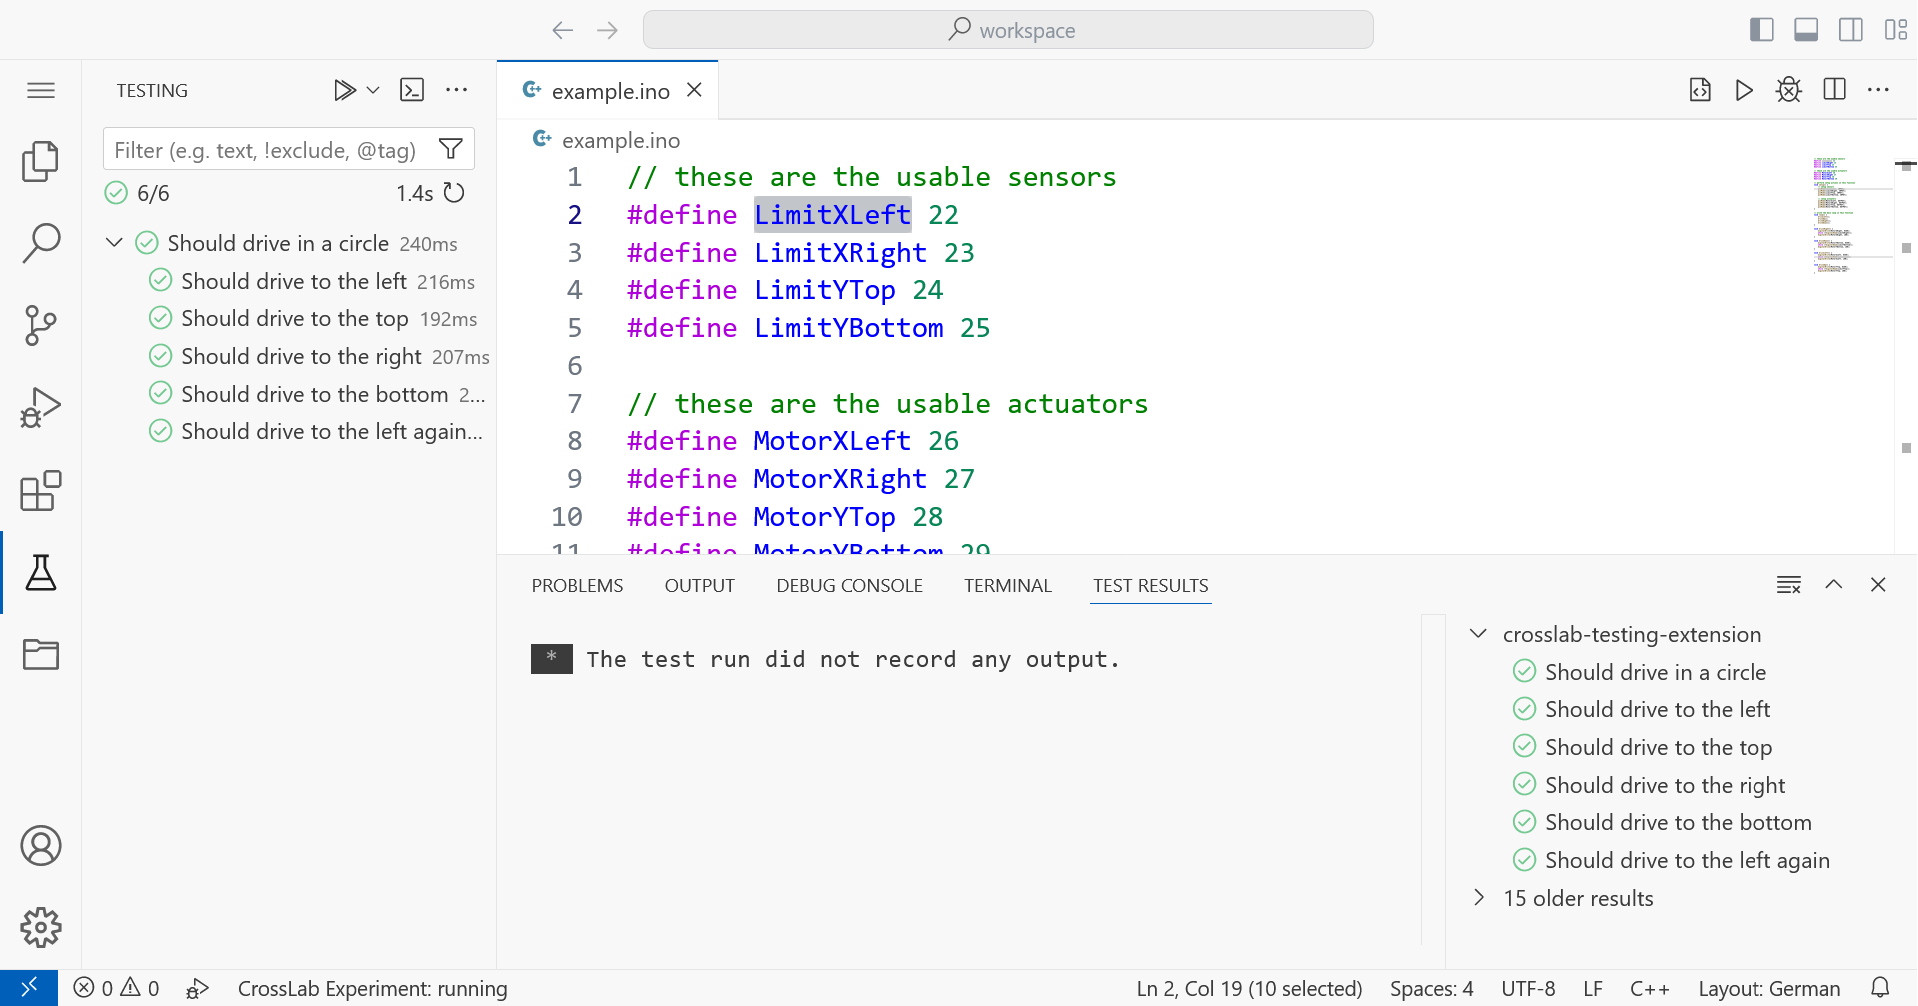
\includegraphics[trim={0 3px 0 0},clip,width=\textwidth]{images/tests-success.png}
    \caption{Benutzerinterface für die Ausführung von Testfällen}
    \label{figure:benutzerinterface:testen}
\end{figure}

Für die IDE wurde eine entsprechende Erweiterung implementiert. Diese wird im Folgenden als \textit{Testing Erweiterung} bezeichnet und stellt einen Testing Service Consumer bereit. Weiterhin wird die VSCode Testing API, ein Teil der VSCode Extension API, verwendet, um die Testfälle in der IDE anzeigen und ausführen zu können. Dabei wird das bereits in VSCode enthaltene Benutzerinterface für Tests verwendet. Dieses ist in \autoref{figure:benutzerinterface:testen} dargestellt.

Der betrachteten Experimentkonfiguration wird kein neues Laborgerät hinzugefügt. Jede IDE wird um einen Testing Service Consumer und die Steuereinheit um einen Testing Service Producer erweitert. Zudem stellt die Steuereinheit Funktionen zum Setzen und Auslesen der Pins des simulierten Microcontrollers zur Verfügung. Es werden Verbindungen zwischen den IDEs und der Steuereinheit über den Testing Service hinzugefügt (sh. \autoref{figure:experimentkonfiguration:testen}).
\section{Language Server}\label{section:prototypische-implementierung:language-server}

% \begin{note}
%     \textbf{Notizen:}
%     \begin{itemize}
%         \item Begründung warum Arduino Language Server genutzt wurde
%         \item Anbindung des Arduino Language Server als Laborgerät
%         \item Beschreibung der implementierten VSCode Erweiterung
%         \item Beschreibung der aufgetretenen Probleme und deren Lösung
%     \end{itemize}
% \end{note}

Für die prototypische Implementierung wurde ein cloud-instanziierbares Laborgerät für die Bereitstellung des \textit{Arduino Language Servers} \cite{noauthor_arduino-language-server_2025} implementiert. Dieses besitzt einen entsprechenden Language Server Service Producer. Wenn die IDE den Language Server startet, schickt sie zunächst die entsprechende Initialisierungsnachricht mit dem aktuellen Projekt des Nutzers. Dieses wird auf der Seite des Language Server gespeichert. Danach wird der Language Server gestartet und eine Antwort an die IDE gesendet. Diese kann daraufhin mit der Ausführung des \ac{LSP} beginnen. Dabei muss auf der Seite des Language Servers eine Anpassung der URIs für eingehende und ausgehende \ac{LSP} Nachrichten erfolgen. Dies kann auf eine ähnliche Weise erfolgen, wie es bereits in \autoref{section:prototypische-implementierung:debugging} für das \ac{DAP} beschrieben wurde.

Für die IDE wurde eine entsprechende Erweiterung entwickelt. Diese wird im Folgenden als \textit{Language Server Erweiterung} bezeichnet und stellt einen Language Server Service Consumer bereit. Wenn eine Verbindung für diesen besteht, wird der entsprechende Language Server gestartet und über den VSCode Language Client angebunden. Weiterhin wurde ein \texttt{TextDocumentContentProvider} implementiert, der in Verbindung mit dem Language Server Service Consumer den Lesezugriff auf die lokalen Dateien des Language Servers ermöglicht.

Die betrachtete Experimentkonfiguration wird um das neue Laborgerät für die Bereitstellung des Arduino Language Servers erweitert. Dieses wird über den Language Server Service mit den IDEs verbunden.